\section{Input Supply Filter} \label{subsec:SupplyFilter}

The $\pm 15V$ supply on figure \refq{fig_7_1_6_DCSUPPLY} is coming from a Mean Well RT65C switching converter. To reduce switching noise in the input for the analog supply, a small filter has been added to the input, as can be seen on the right side of figure \refq{fig_7_1_6_DCSUPPLY}. The filter is designed as a second order system with a damping resistor and with a pre-chosen inductor of $L = 1E-3$H as shown on the schematic on figure \refq{fig_7_1_5_SupplyFilterSch}.

\begin{figure}[H]
    \centering
    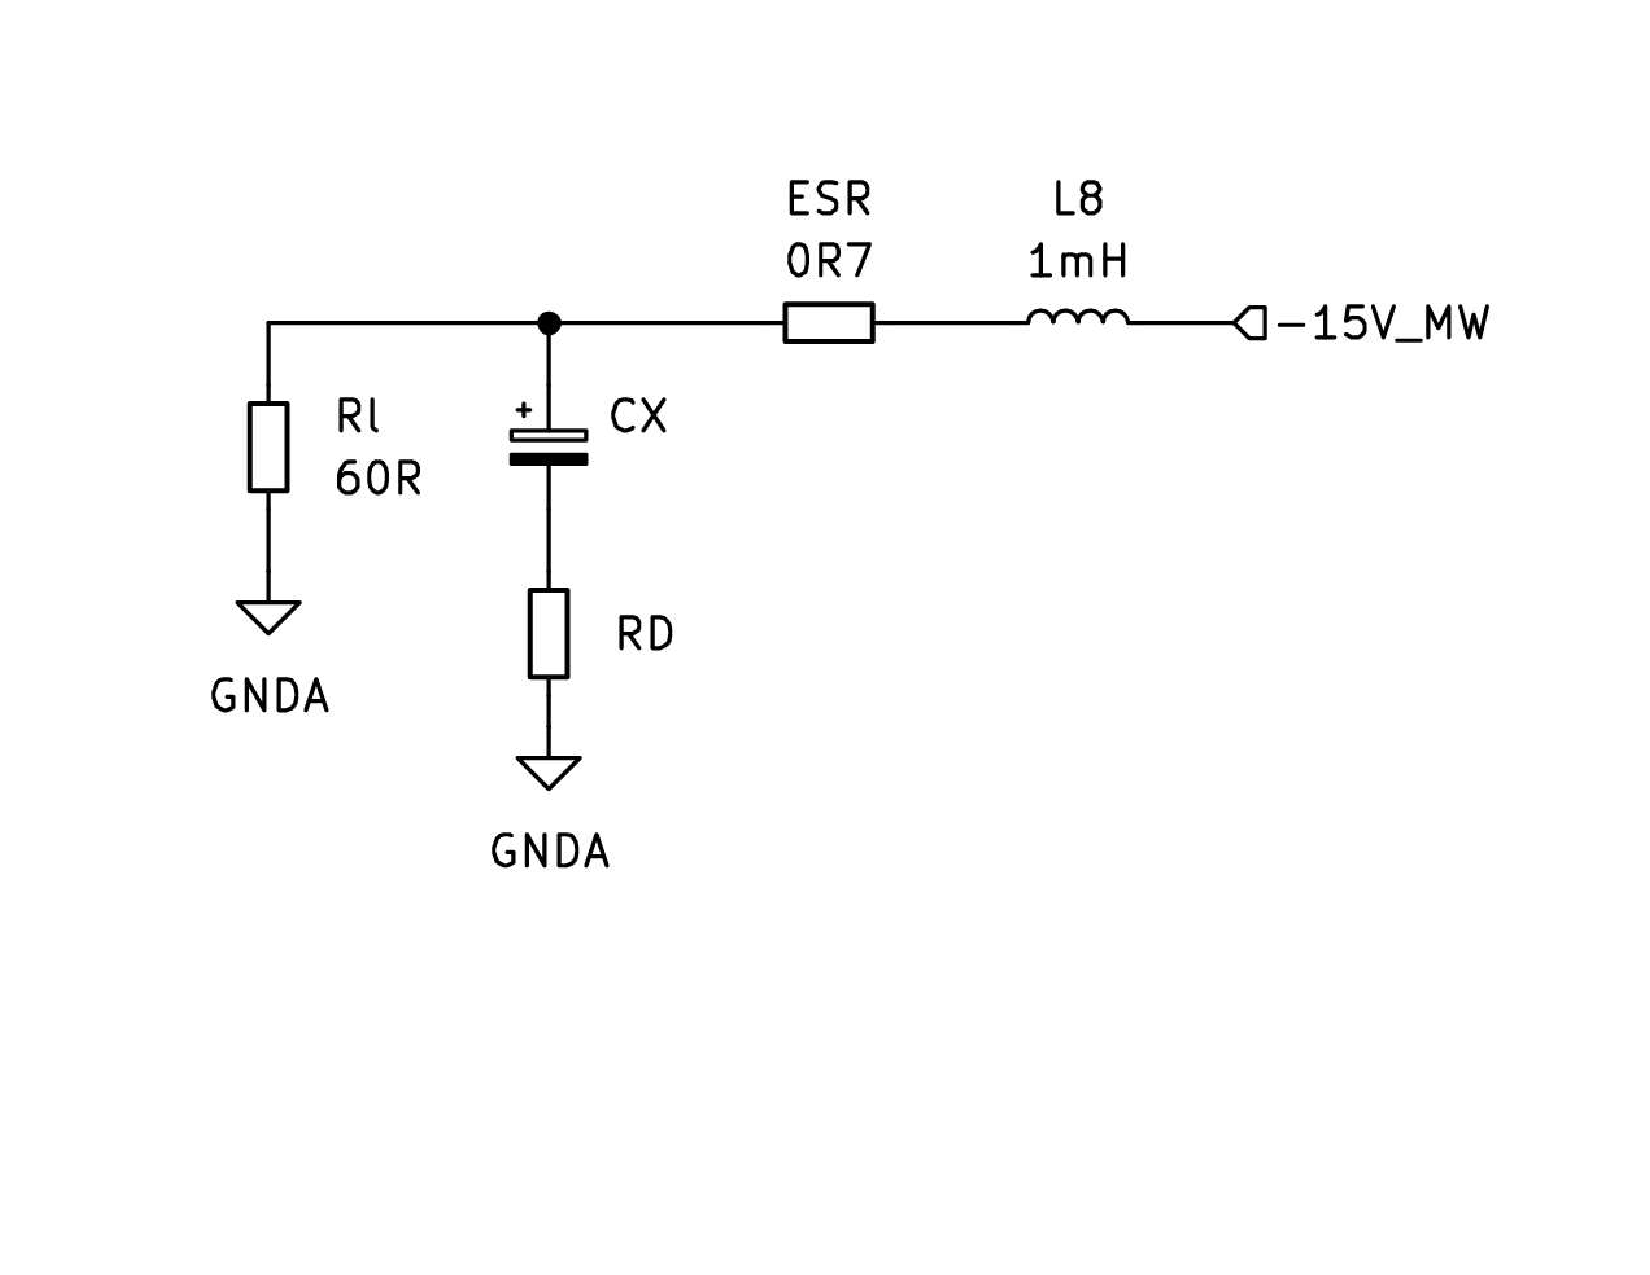
\includegraphics[clip, trim=0 150 0 0, width=0.75\textwidth]{Sections/7_SystemDesign/Figures/7_1_5_SupplyFilterSch.pdf}
    \caption{The input filter prototype for the DC supply. The inductor L8 corresponds to L1 and L2 on figure \refq{fig_7_1_6_DCSUPPLY} and is a component that was chosen before hand.}
    \label{fig_7_1_5_SupplyFilterSch}
\end{figure}

The output is across the load impedance marked as $R_L$ and the transfer function for this circuit can be found as a simple voltage divider as shown in equation \refq{eq:7_1_5_FILTF}.

\begin{equation}\label{eq:7_1_5_FILTF}
    A_V = \frac{    \frac{     (\frac{1}{sC} + R_{DC})R_L     }{  \frac{1}{sC} + R_L + R_{DC}  }      }{ \frac{     (\frac{1}{sC} + R_{DC})R_L     }{  \frac{1}{sC} + R_L + R_{DC}  }   + sL + R_{DL}}
\end{equation}

The transferfunction \refq{eq:7_1_5_FILTF} can, after a bit of work, be re-written to the form in eq \refq{eq:7_1_5_FILTF2}. It is evident that this is an ordinary second-order system.
\begin{equation}\label{eq:7_1_5_FILTF2}
    A_V = \frac{   \frac{(R_{DC}Cs + 1)R_L}{CL(R_L+R_{DC})}}{s^2 + \frac{(((R_{DC}+R_{DL})R_L + R_{DC}R_{DL})C+L)}{CL(R_L + R_{DC})}s + \frac{R_L}{CL(R_L + R_{DC})} + \frac{R_{DL}}{CL(R_L + R_{DC})}} 
\end{equation}

A general second-order system is of the form shown in equation \refq{eq:7_1_5_GENTF}. 

\begin{equation}\label{eq:7_1_5_GENTF}
    A_V = \frac{\omega_n^2}{s^2 + 2\zeta\omega_ns+\omega_n^2}
\end{equation}

By comparing eq \refq{eq:7_1_5_FILTF} and eq \refq{eq:7_1_5_GENTF} it can be seen that the following terms in \refq{eq:7_1_5_TFFACTORS}are equal.
\begin{equation}\label{eq:7_1_5_TFFACTORS} 
    \begin{aligned}
        2\zeta\omega_n = \frac{(((R_{DC}+R_{DL})R_L + R_{DC}R_{DL})C+L)}{CL(R_L + R_{DC})} \\
        \omega_n^2 = \frac{R_L}{CL(R_L + R_{DC})} + \frac{R_{DL}}{CL(R_L + R_{DC})}
    \end{aligned}
\end{equation}

The natural frequency, $\omega_n$, for the system is \refq{eq:7_1_5_NATFRQ}.
\begin{equation}\label{eq:7_1_5_NATFRQ}
    \omega_n = \sqrt{\frac{R_L}{CL(R_L + R_{DC})} + \frac{R_{DL}}{CL(R_L+R_{DC})}}
\end{equation}
The damping factor, $\zeta$ is, after a bit of work, shown in equation \refq{eq:7_1_5_DAMPF}.
\begin{equation}\label{eq:7_1_5_DAMPF}
    \zeta = \frac{C(R_{DC}+R_{DL})R_L + CR_{DC}R_{DL} + L}{2\sqrt{\frac{R_L +R_{DC}}{CL(R_L + R_{DC})}}CL(R_L+R_{DC})}
\end{equation}

The MW RT65C is switching at \SIQ{60}{\kilo\hertz}, so the natural frequency of the system will be set to a significantly lower value than this. $\omega_n = 200\pi$, or \SIQ{100}{\hertz}, has been arbitrarily chosen. To imitate a low-pass response the damping factor will be chosen to produce an overdamped response, so, $\zeta$ > 1. Several values were tested, this will not be shown, and $\zeta = \sqrt{2}$ will produce the desired low-pass response. Reducing the value of $R_D$ will give damping factor values of $\zeta < 1$ and cause the system to give an underdamped response with gain peaking near the natural frequency, this is undesirable for a low pass filter.

Using $\omega_n = 200\pi$ and equation \refq{eq:7_1_5_NATFRQ} an expression for the capacitor can be found. The inductor was pre-chosen and has the values $L = 1E-3$H with series resistance $R_L = 710E-3\Omega$. Using appendix \refq{App:PowerConsumption} for the power consumption on the 12V rail, the expected load is about $R_L = 60 \Omega$. The result can be seen in eq \refq{eq:7_1_5_COMP1}.

\begin{equation}\label{eq:7_1_5_COMP1} 
    \begin{aligned}
        \omega_n = \sqrt{\frac{R_L}{CL(R_L + R_{DC})} + \frac{R_{DL}}{CL(R_L+R_{DC})}}\\
        200\pi = \sqrt{\frac{60}{C\cdot 1E-3 \cdot(60 + R_{DC})} + \frac{0.7}{C\cdot 1E-3 \cdot (60 + R_{DC})}}\\
        C = \frac{0.1538}{60 + R_{DC}}
    \end{aligned}
\end{equation}

The result from eq \refq{eq:7_1_5_COMP1} will be denoted as $C_X = C$ and used in equation \refq{eq:7_1_5_COMP2}. Using $\zeta = \sqrt{2}$ in the equation for the damping factor \refq{eq:7_1_5_DAMPF}, a value for the damping resistor, $R_D$, can be found as shown in eq \refq{eq:7_1_5_COMP2}.

\begin{equation}\label{eq:7_1_5_COMP2} 
    \begin{aligned}
        \zeta = \frac{C_X(R_{DC}+R_{DL})R_L + C_XR_{DC}R_{DL} + L}{2\sqrt{\frac{R_L +R_{DC_X}}{CL(R_L + R_{DC_X})}}C_XL(R_L+R_{DC_X})}\\
        \sqrt{2} = \frac{  \frac{(R_{DC} + 0.7)60 + R_{DC}\cdot 0.7 + 1e-3}{C_X \cdot 1e-3(60 + R_{DC})}  }{2\sqrt{ \frac{60}{C_X \cdot 1e-3 \cdot (60+R_{DC})} + \frac{0.7}{C_X \cdot 1e-3 \cdot (60+R_{DC})} }}\\
        R_{DC} = 1.0795
    \end{aligned}
\end{equation}

The value for $R_D$ can be substituted back into equation \refq{eq:7_1_5_COMP1} to find the value for C as shown in eq \refq{eq:7_1_5_COMP3}.
\begin{equation}\label{eq:7_1_5_COMP3} 
    \begin{aligned}
        C = \frac{0.1538}{60 + R_{DC}}\\
        C = \frac{0.1538}{60 + 1.07946}\\  
        C = 0.002489
    \end{aligned}
\end{equation}

The values for $C$ and $R_D$ will produce an overdamped response as shown on the simulation output on figure \refq{fig_7_1_5_SupplyFilterSimOut}.
\begin{figure}[H]
    \centering
    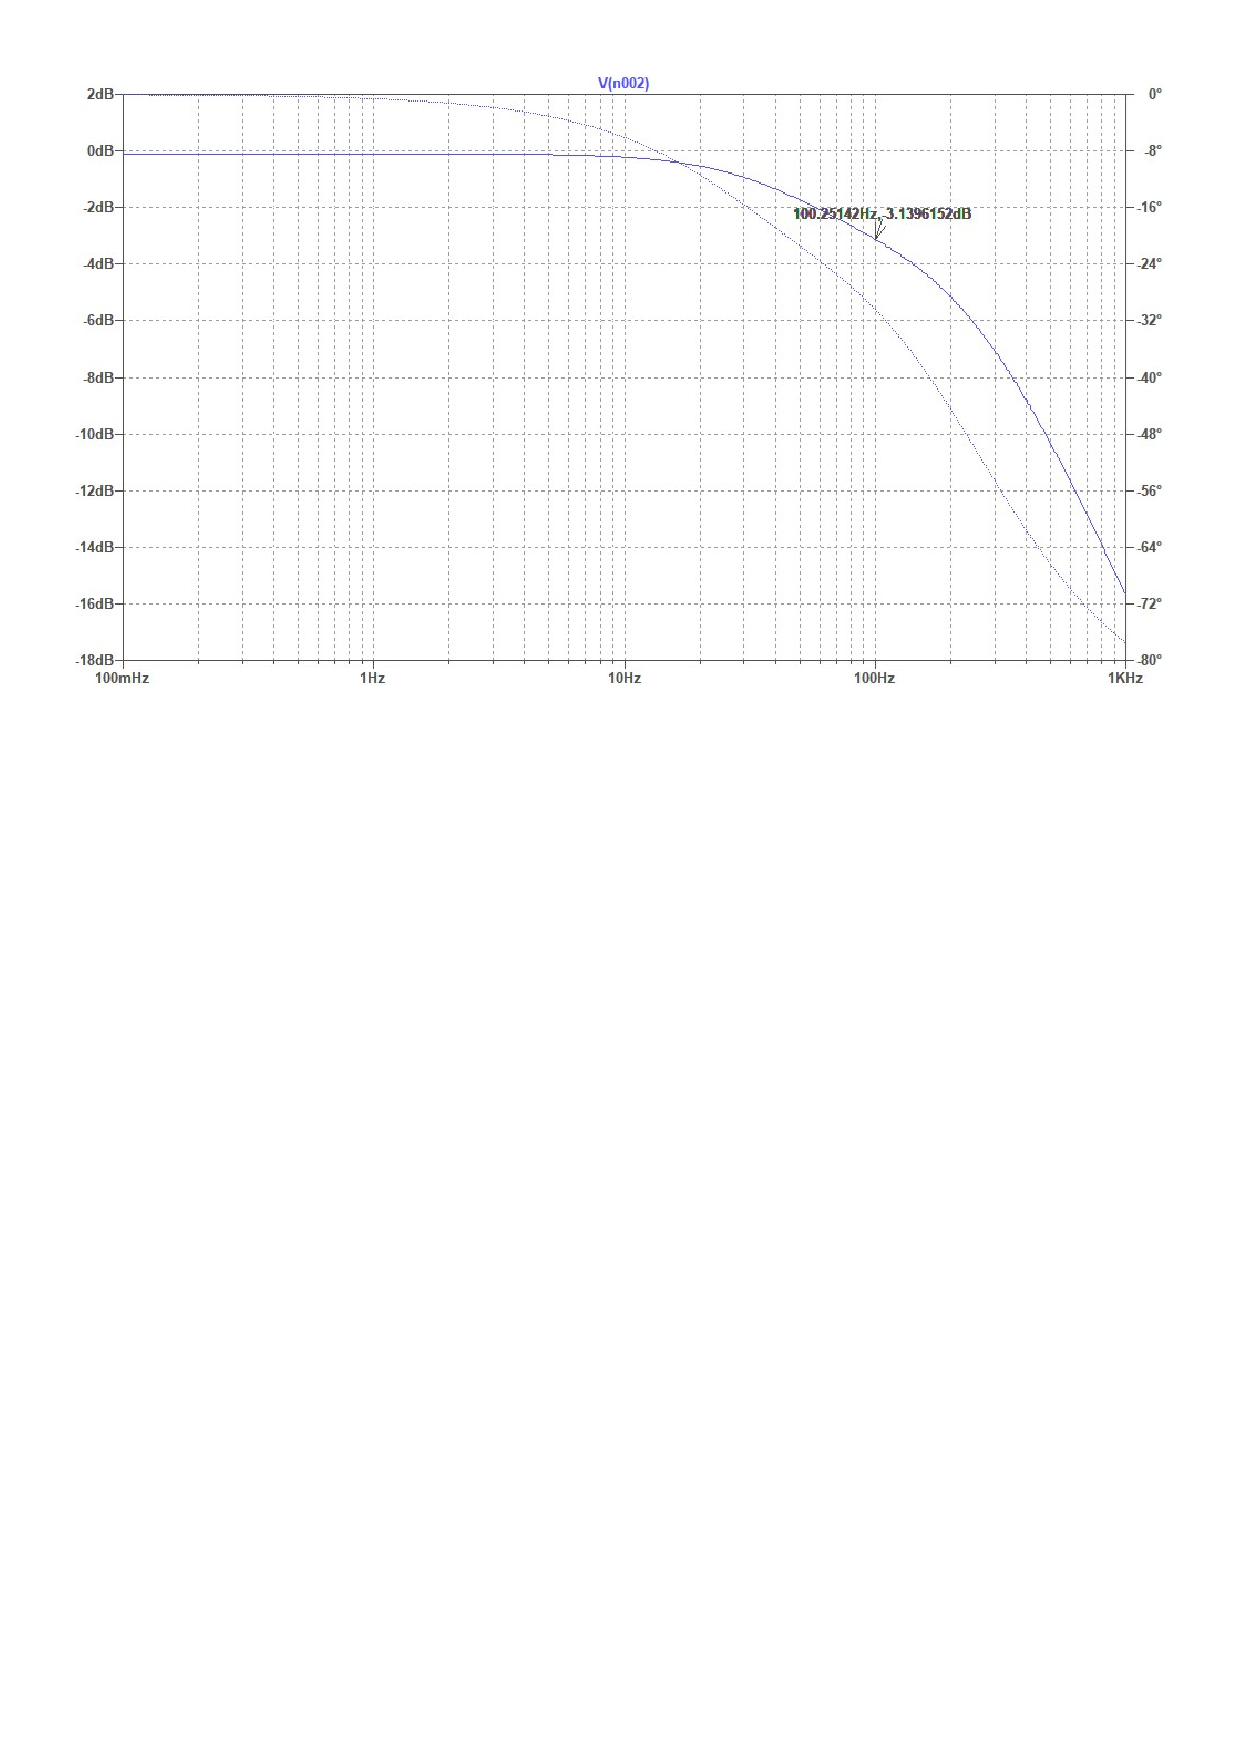
\includegraphics[clip, trim=0 500 0 0, width=1\textwidth]{Sections/7_SystemDesign/Figures/7_1_5_SupplyFilterSimPlot.pdf}
    \caption{The simulation output for the circuit shown in figure \refq{fig_7_1_5_SupplyFilterSch} with the values that were found for the damping resistor and capacitor. Note how the -3dB cut-off for the low pass filter is close to the natural frequency of 100Hz for the overdamped system.}
    \label{fig_7_1_5_SupplyFilterSimOut}
\end{figure}

 The low-pass filter could also have been designed and realized as a ladder structure after frequency scaling. This was initially attempted, but the filters made through this method produced far too large inductance values for a filter with a cut-off close to DC (100s of mH), so the method shown in this section was used instead. The inductor was chosen based on cost and availability as capacitors are significantly cheaper components. The results from this approach is more in line with the projects overall goals.